\documentclass{article}
\usepackage{fontspec}

% Used to embed Sage code in latex
%\usepackage{sagetex}


% Math Environment
\usepackage{euler}        % Euler font
\usepackage{amsmath}      % Math macros
\usepackage{amssymb}      % Math symbols
\usepackage{unicode-math} % Unicode support

% Physics Environment
\usepackage{physics}


\usepackage[makeroom]{cancel} % Used to cancel terms in algebraic equations
\usepackage{ulem} % Different underline environments
\usepackage{polynom} %Polynomial long division

% Typesetting Rules
\setlength\parindent{0em}
\setlength\parskip{0.618em}
\usepackage[a4paper,lmargin=1in,rmargin=1in,tmargin=1in,bmargin=1in]{geometry}
\setmainfont[Mapping=tex-text]{Helvetica Neue LT Std 45 Light}

% Common Macros
\newcommand\N{\mathbb{N}}
\newcommand\Z{\mathbb{Z}}
\newcommand\Q{\mathbb{Q}}
\newcommand\R{\mathbb{R}}
\newcommand\C{\mathbb{C}}
\newcommand\A{\mathbb{A}}
\def\res{\mathop{\text{Res}}\limits}

% Color
\usepackage[dvipsnames]{xcolor}
\usepackage{pagecolor}
% \definecolor{DeepMossGreen}{HTML}{394820}
% \pagecolor{DeepMossGreen}
% \color{Goldenrod}

\usepackage{graphicx}

\begin{document}

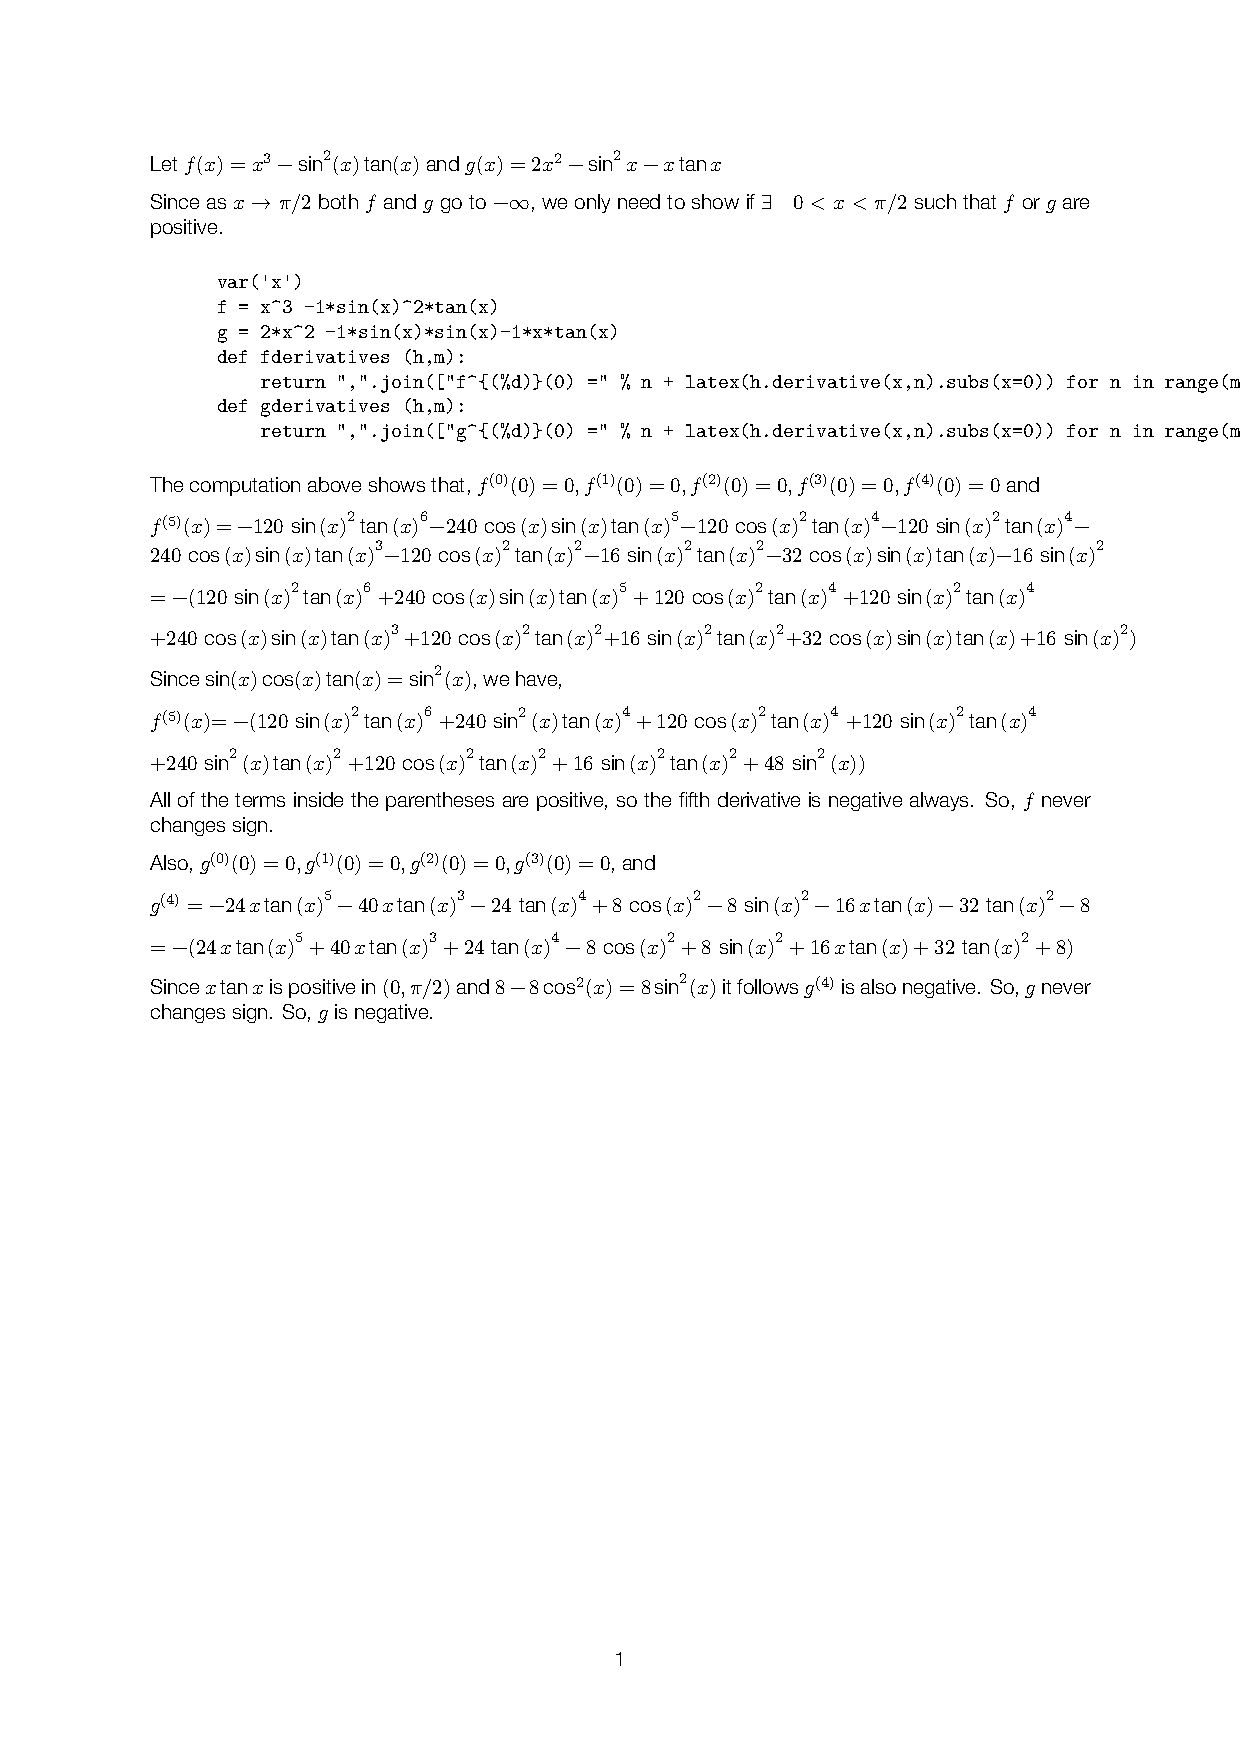
\includegraphics[width=\textwidth]{q2.png}
\uwave{slu.}

Since $\sin(1/t)$ is bounded we have,
\[f(0) = \lim_{t\rightarrow 0 } t + 2\cdot t^2 \sin(1/t) = 0\]

By the definition of the derivative,
\[f'(0) = \lim_{t\rightarrow 0} \frac{f(0+t) -f(0)}{t} =
  \lim_{t\rightarrow 0} \frac{t +2t^2 \sin(1/t)}{t} = 1\]

Computing the derivative we get,
\[f'(t) = 1 + 4t\sin(1/t) -2\cos(1/t)\]

Then for $t \in (-1,1)$,

\begin{equation*}|f'(t)| = |1 + 4t\sin(1/t) -2\cos(1/t)|
  \leq 1 +4+2 = 7
\end{equation*}

So $f'$ is bounded in $(-1,1)$.

$\forall n\in \Z: n\neq 0$, let $a_n  = 2n\pi$ and $b_n = (2n+1)\pi$, then

\[f'(1/a_n) = 1 + 4\frac{1}{2n\pi}\sin(2n\pi) -2\cos(2n\pi) = 1 -
  2 = -1\]
\[f'(1/b_n) = 1 + 4\frac{1}{(2n+1)\pi}\sin((2n+1)\pi)
  -2\cos((2n+1)\pi) = 1 + 2 =3\]

It follows that $f$ has a local
maximum on $(1/b_n,1/a_n)$ and a local minimum on $(1/a_n,1/b_{n-1})$.

Since every neighborhood of $0$ contains infinitely many of such
intervals, it follows that $f$ cannot be injective in any neighborhood
of $0\quad \lozenge$

\end{document}



%%% Local Variables:
%%% mode: latex
%%% TeX-master: t
%%% End:
